\section{Frame invariance and an information leak in a fixed-origin simulation}
\label{app:leak}
Simulations frequently place the lens at the coordinate origin. If absolute image coordinates are then given to a trained estimator, it can measure the image radii from the exact lens centre and so bypass the error of the measured centre: the inputs contain information that real data do not provide. We quantified this effect on an earlier, smaller benchmark of 2500 selected SIS events (ET-D, $0.05<z_s<1.5$) in which the true centre was fixed at the origin and the inputs contained absolute image and centre coordinates. With otherwise identical HistGB settings and ten random divisions into training, calibration and test events (1750/375/375), replacing the absolute coordinates by translation-invariant inputs raised the MAE of the geometry-only estimate from $0.193\pm0.038$ to $0.270\pm0.040$, and that with all inputs from $0.207\pm0.041$ to $0.239\pm0.036$. A Bayesian SIS posterior from the image coordinates, marginalised over the unknown centre, attains MAE $0.243\pm0.032$ on the same events: it beats the corrected estimator, as it should for a correct lens model, whereas the estimator with absolute coordinates appeared to beat it. In the same earlier study, images in the non-SIS benchmark had been ordered by their true magnification, which reveals the target whenever more than two images exist. All results in this paper use a random true centre and frame rotation, inputs that are invariant under translations and rotations, and images ordered by measured SNR.

\section{Additional results}
\label{app:extra}
Fig.~\ref{fig:learning} shows the median relative error as a function of the number of training events for SIS and SIE+shear lenses (ET). The errors stop decreasing above $\sim10^4$ events. The results are therefore not limited by the size of the ET training sets (36\,000 events per family), while the O5 samples (900--1800 training events per family) lose about 1--2 percentage points relative to the asymptotic accuracy.

\begin{figure}
\centering
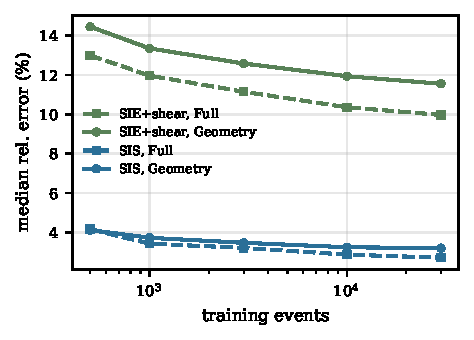
\includegraphics[width=\columnwidth]{fig_learning.pdf}
\caption{Median relative error of $\mu_A$ versus the number of training events for ET.}
\label{fig:learning}
\end{figure}

